\documentclass{sig-alternate}
\usepackage{url}
\usepackage{pgffor}
\usepackage{subcaption}
\usepackage{comment}
\usepackage{graphicx}% http://ctan.org/pkg/graphicx
\usepackage[usenames,dvipsnames,svgnames,table]{xcolor}


%http://www.esa.int/gsp/ACT/doc/ARI/ARI%20Study%20Report/ACT-RPT-AI-ARI-12-5201-Space%20Gaits.pdf
%http://www.esa.int/gsp/ACT/doc/AI/pub/ACT-RPR-AI-2013-spacegaits.pdf
%hildebrand diagrams

%introduction - related
%background
%methodology - novelty, 
%behavior
%temp cycle of meteorites, can actuate materials, future simulator
%multiple behaviors

\usepackage{etoolbox}
\apptocmd{\thebibliography}{\small}{}{}
\usepackage{setspace}

\begin{document}

 \conferenceinfo{GECCO'15,} {July 11-15, 2015, Madrid, Spain.}
    \CopyrightYear{2015}
    \crdata{TBA}
    \clubpenalty=10000
    \widowpenalty = 10000

\title{Novelty Search for Soft Robotic Space Exploration}
%\subtitle{[Extended Abstract]
%\titlenote{A full version of this paper is available as
%\textit{Author's Guide to Preparing ACM SIG Proceedings Using
%\LaTeX$2_\epsilon$\ and BibTeX} at
%\texttt{www.acm.org/eaddress.htm}}}

\numberofauthors{1}
\author{
\alignauthor
		Georgios Methenitis, Daniel Hennes*, Dario Izzo*, Arnaud Visser**\\
       \affaddr{Centrum Wiskunde \& Informatica, Amsterdam}\\
       \affaddr{*European Space Agency}\\
       \affaddr{**University of Amsterdam}\\
       \email{georgios.methenitis@cwi.nl, daniel.hennes@esa.int, dario.izzo@esa.int, a.visser@uva.nl}
}

\maketitle
\begin{abstract}
Soft robotics is a vivid research field on the science and engineering aspects of soft materials in mobile machines. Recent development in soft robotics and evolutionary optimization have shown the ability to simultaneously evolve the morphology and locomotion of soft robots. Generative encoding coupled with neural evolution of augmented topologies shows promising results. Novelty search, unlike traditional optimization methods does not aim to optimize the objective but instead looks for novelty. Novelty search rewards diversity and leads to a variety of solutions, mimicking natural evolution. Apart from the performance comparison between novelty and fitness based search, this paper shows that new locomotion patterns can be produced by the former while different types of selection algorithms for fitness and novelty based evolution are studied. In addition, a method to combine both is proposed. Finally, the objective-wise performance is tested under variant gravity conditions leading into a taxonomy of possible locomotion strategies given different gravity levels.
\end{abstract}

% A category with the (minimum) three required fields
\category{H.4}{Information Systems Applications}{Miscellaneous}
%A category including the fourth, optional field follows...
%\category{D.2.8}{Software Engineering}{Metrics}[complexity measures, performance measures]

\terms{Theory}

\keywords{soft robotics, novelty search, CPPN, CPPN-NEAT, HyperNEAT, VoxCAD, space exploration}

\section{Introduction}
Space exploration in regards to unmanned missions for close physical investigation of celestial bodies in our solar system remains a very tough task for space engineering, considering the current level of space technology, where the only power sources are either limited to a certain lifespan or depend on sunlight availability while traditional ways of locomotion are limited and sometimes unable to produce locomotion on different gravity levels. For this reason, gravity conditions play a major role in the design and performance aspects of rigid body robots. For example, the Mars rover~\cite{grotzinger2012mars} (Curiosity) design followed a traditional car-like shape and size, its mobility systems depend on six-wheel system that can drive the rover on Mars' surface. More recently, European Space Agency (ESA) successfully achieved to land a rigid probe on the surface of the comet 67P/Churyumov-Gerasimenko (67P). The probe is believed that bounced twice on the surface of the comet before finally landed in a rough terrain going into hybernation due to insufficient sunlight to power its systems, and the inability to perform any kind of movement. In this paper, we investigate ways to the evolution of the design of soft robotic bodies that can be passively actuated on different levels of gravity. We are interested in applying evolutionary techniques to evolve the morphology of soft robots that can inspire future robotic missions, as well as to build on top of previous work applying a search technique known as \emph{Novelty Search} to the evolution of soft robotic morphology and locomotion strategy.

\subsection{Soft Robots}

\begin{figure}[t!]
\centering
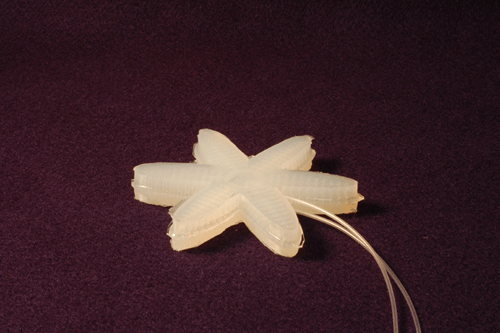
\includegraphics[width=0.22\textwidth,height=0.12\textheight]{../Figures/Misc/soft_robotics_figure.png}\		
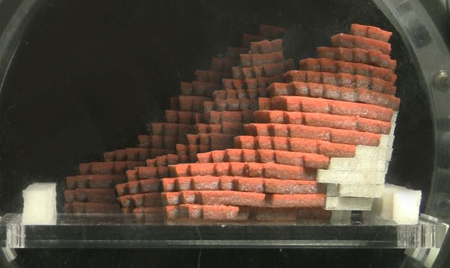
\includegraphics[width=0.22\textwidth,height=0.12\textheight]{../Figures/Misc/hillerPressureChamber.png}\\[0.1cm]	
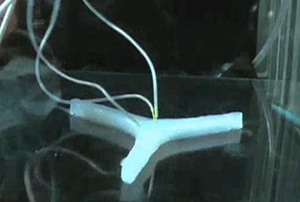
\includegraphics[width=0.22\textwidth,height=0.12\textheight]{../Figures/Misc/ExplodingRobot.jpg}\	
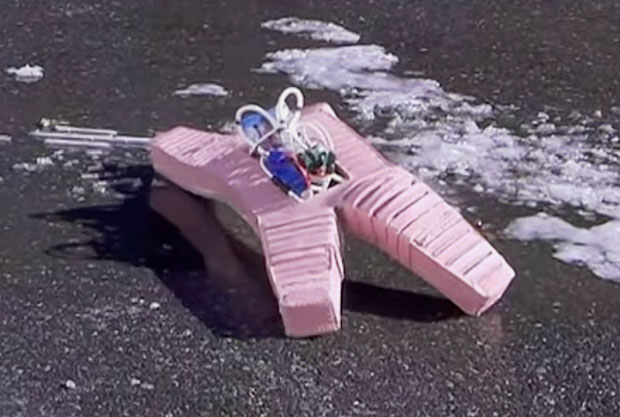
\includegraphics[width=0.22\textwidth,height=0.12\textheight]{../Figures/Misc/softbot.jpg}\\
\caption{Soft robots can be actuated through air pressure tubes (top-left), pressure variations (top-right), or internal explosions (bottom-left). Autonomously actuated soft robot~\cite{tolleyresilient}, it is able to withstand extreme temperatures and variant terrain types (Bottom-right).}
\label{fig:softRobotsActuation}
\vspace{-15pt}
\end{figure}

Soft robotics is a highly promising field of research dedicated to the science and engineering of soft materials in mobile machines. As the name suggests soft robots~\cite{trivedi2008soft, pfeifer2012challenges} are made entirely of soft materials mimicking animals or animal-parts that consist only of soft tissue (elephant trunk, tongue, worm, octopus, etc.). Having no rigid parts in their design the degrees of freedom are infinite and the possible ways of motion can become extremely complex. In traditional robotics, joints and rigid parts predefine the space of possible movement and sometimes restrict the robot's locomotion strategy or \emph{gait} to a specific set. In soft robotics, the absence of rigid parts can on the one hand make the design of the locomotion strategy exceptionally tortuous, on the other hand the gait alternatives are limitless.

The actuation of such soft structures is the most challenging task. Actuating soft materials can be done in many ways including pneumatic systems~\cite{ilievski2011soft, shepherd2011multigait}, hydraulic, internal body explosions, passive actuation triggered by pressure or temperature variations and others~\cite{laschi2012soft, seok2010peristaltic}. Figure~\ref{fig:softRobotsActuation} illustrates four different ways that soft robot bodies can be actuated. Autonomously actuated soft robots~\cite{tolleyresilient} can also be designed having multiple advantages over rigid body robots such as resistance under extreme temperatures and the capability of locomotion on terrains of variant types.

\subsection{Evolution of robotic locomotion}

Evolutionary algorithms have been used to evolve the locomotion strategy of rigid and soft robots. Furthermore, the effects of gravity have been studied showing that it is possible to obtain a set of parameters to stabilize the gaits of a rigid robot under different levels of gravity.

Complex encoding representations such as artificial neural networks can control not only the morphology of rigid body parts connected with joints, but also control the forces applied to each joint. As a result, virtual creatures can be produced in a physical three-dimensional world~\cite{sims1994evolving}. Methods for evolving such virtual creatures like in~\cite{sims1994evolving} can utilize novelty search~\cite{lehman2011evolving} and be far more explorative in the space of morphologies. Behavior novelty defined as a measure between morphological properties of the produced creatures driving the evolution to explore more diverse morphologies.

\subsubsection*{The effects of gravity on rigid robot gait evolution for space missions}

The effects of gravity, slopes, and stiffness to the gaits achieved by a quadruped robot in dynamic walking and running have been researched~\cite{papadopoulos2013ariadna, kontolatisquadruped}. Furthermore, Hildebrand gait diagrams~\cite{hildebrand1989quadrupedal} are employed in analysing gaits resulting from an optimisation process according to criteria important for space missions, such as motion speed and energy efficiency. This study showed that it is possible to obtain stable gaits despite the varied conditions encountered in planetary exploration.

\subsubsection*{Evolution of soft robots}

Considering soft robotics, topological optimization techniques can be applied to soft robots~\cite{hiller2009multi} for producing functionality in the design. Evolution of soft material robots as it was shown in~\cite{hiller2012automatic}, can result in soft robots able to produce locomotion. The possibility of evolving these soft structures using an indirect encoding was of interest to be exploited by~\cite{cheney2013unshackling}. A powerful generative encoding, CPPNs~\cite{stanley2007compositional}, was used to generate soft voxel-formed three-dimensional structures, coupled with the use of NEAT algorithm which ensures the increasing complexity of the networks produced. The superiority of this kind of generative encoding was verified against direct encoding, showing how CPPNs can take advantage of their geometrical properties. Evaluation was done by a simple displacement measure while evolution tended to evolve different kinds of locomotion strategies and morphologies as the fitness function was penalized for different parameters. An earlier work~\cite{hiller2010evolving}, apart from the generative encoding of CPPNs, made use of \textit{Gaussian Mixture} and \textit{Discrete Cosine Transform} to produce amorphous soft body structures. The simultaneous evolution of soft robot morphology and control was also investigated by recent work~\cite{rieffel2014growing}. Some aspects of soft robot evolution were verified in this work, namely muscle placement and muscle-firing patterns can be evolved given a fixed body shape and fixed material properties. Furthermore, material properties can be co-evolved alongside locomotion strategies.

The present work builds upon previous work~\cite{cheney2013unshackling} making also use of novelty search to co-evolve the morphology and the locomotion capability of soft bodied virtual creatures. Pure novelty search failed to evolve fit solutions in previous work~\cite{lehman2011evolving} used, it is of interest to apply and investigate its performance in virtual soft robots this time. We also investigate the effects of gravity in the evolution of soft robots morphology and locomotion strategy for the first time in the evolution of soft robotics. 

\section{Background}

\subsection{VoxCAD simulator}

Most work to simulate interactions and deformations within and between soft material bodies are mostly focused on the graphical part of the problem~\cite{faloutsos1997dynamic} sacrificing the accuracy of the simulation~\cite{teschner2004versatile}. Three dimensional meshes~\cite{muller2002stable} can represent these bodies including the dynamics of their materials. \emph{VoxCad} simulator~\cite{hiller2012dynamic}, is focusing mostly on the physics side of the soft material interactions not at the expense of a low frame rate simulating soft material deformations and interactions. A lattice is used within the simulator to represent the 3D workspace where voxels can be assigned different materials. Materials themselves are passive and cannot actuate without external trigger. The external force that can actuate the materials is the temperature of the environment.

\subsubsection*{Materials}

Materials can be \emph{passive} or \emph{active} in respect to their reaction to the temperature changes. Passive materials do not react to temperature changes, while active materials expand and contract in respect to their thermal properties. \textcolor{Red}{Red} and \textcolor{Green}{Green} are the only actuated materials with non-zero and opposite thermal expansion coefficients. The two additional materials represent non-actuated tissue that can be soft (soft tissue) or hard (bones). \textcolor{Cyan}{Cyan} voxels are soft having five times smaller elastic modulus of their material than \textcolor{Blue}{Blue} which have $50$ \texttt{MPa}.

\begin{figure}[t!]
\centering
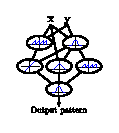
\includegraphics[width=0.15\textwidth]{../Figures/Misc/cppnNetwork.eps}
\caption{Compositional pattern-producing networks have identical network structure with artificial neural networks while they make use of a canonical set of activation functions.}
\label{fig:cppnNetwork}
\vspace{-15pt}
\end{figure}


\subsection{Compositional Pattern-Producing Networks}



\emph{Compositional pattern-producing networks} (CPPNs)~\cite{stanley2007compositional} are artificial neural networks with an extended set of activation functions (see Fig.~\ref{fig:cppnNetwork}). This set of activation functions include repetitive, symmetrical, and linear functions. CPPNs can generate phenotypes that can be interpreted as distributions of points in a multidimensional Cartesian space, networks can then be queried in multiple resolutions.

\begin{figure}[b!]
\centering
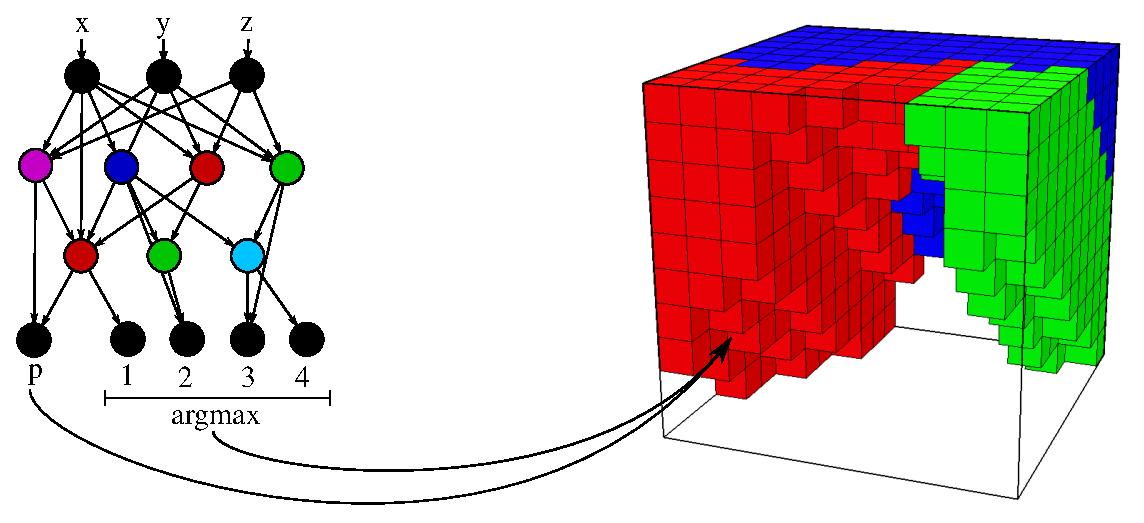
\includegraphics[width=0.35\textheight]{../Figures/Misc/cppnSoftBot.eps}
\caption{Each genotype (CPPN) is queried for every coordinate inside the lattice, its outputs determine the presence of a voxel and the type of its material.}
\label{fig:cppnDiagram}
\vspace{-15pt}
\end{figure}

For the purpose of this work, CPPNs are queried for every coordinate of the lattice space to form a soft robot morphology as well as, to define the distribution of the materials. The input nodes (neurons) of the CPPN are assigned to $x,y,z$ normalized coordinates following~\cite{cheney2013unshackling}, so that:
$x,y,z \in [-1,1]$.
A bias input node is also introduced in the genome CPPN representation, this will allow the network to produce arbitrary outputs different from the defaults when all other inputs values are set to zero. More inputs can be added to the CPPNs, for instance the distance from the center point of the Cartesian phenotype space (lattice) as described in~\cite{stanley2007compositional} and used in~\cite{cheney2013unshackling} which adds more bias towards symmetrical structures. The proposed input nodes for the three dimensions of the Cartesian space provide the minimum bias to the network outputs. Figure~\ref{fig:cppnDiagram} illustrates the topology of a random CPPN network with the input and output nodes  described earlier. The presence of a voxel in each coordinate of the lattice is determined by a single output of the CPPN, denoted with $p$ while the selection of the material is determined by $n$-outputs.

\subsection{CPPN-NEAT}

Compositional pattern-producing networks as described earlier are similar computational methods to ANNs in regards to their structure, neuroevolutionary algorithms can be used to evolve CPPNs. NEAT~\cite{stanley2002evolving} method can evolve CPPNs in the place of ANNs, since it only needs few modifications. The resulted method that evolves this generative type of genomes (CPPNs) is called CPPN-NEAT~\cite{stanley2007compositional}. Previous work~\cite{cheney2013unshackling}, showed that this method can indeed evolve the morphologies of the soft robots in the VoxCad simulation environment. \textit{HyperNEAT}\footnote{HyperNEAT \texttt{v4.0 C++}  by J. Gauci code (url: \url{https://github.com/MisterTea/HyperNEAT})} is used for the implementation of the CPPN-NEAT algorithm.

\section{Methodology}

\subsection{Novelty search}

Novelty search~\cite{lehman2008exploiting,lehman2011abandoning,lehman2010revising, risi2009novelty} unlike traditional fitness based search is an alternative way of optimization towards an objective function without having knowledge of this objective. What novelty search seeks for is how interesting a new solution is in respect to all previously found ones. To define ``interesting'' we need to move our point of interest into behavior space which is a function of each phenotype, similar to the fitness function. Nevertheless, it fully or partially describes the behavior without directly implying the fitness function. As an example someone can think of a behavior could be defined as the recorded trajectory of a robot which tries to maximize its velocity. 

To define novelty, a metric measures the difference in the behavior space of the phenotype. Given the phenotype's behavior $x$ a novelty measurement could be a function of $x$, $f(x)$ which computes how different (novel) is the specific behavior in respect to a set of other behaviors $S$ in behavior space.  As defined in~\cite{lehman2008exploiting,lehman2011abandoning} \emph{sparseness} can give a good measurement of how sparse is the area of a newly observed behavior. Given the behavior we can compute the sparseness by:
\begin{equation}
\label{sparsenessEquation}
f(x) = \cfrac{1}{k} \sum_{i=1}^{k} dist(x, S_i)
\end{equation}
where $S$ is a sorted set of the closest behaviors. Sparsity measures the average distance from the $k$-closest behaviors.

One significant point here is that the behavior space in some domains can be limitless. However, a valid behavioral metric can be found excluding behaviors that are meaningless or do not comply with the natural limits of the problem. On the other hand, the search space in the genotype level can also be infinite especially in neuroevolution methods like NEAT where ANNs can grow during the evolution. A bounded space of understandable-valid behaviors is then the key idea of novelty search where increasingly complex behaviors present to the evolution as the complexity of the genotype grows along.

\subsubsection*{Behaviours in Novelty Search}

\begin{figure}[t!]
\centering
\vspace{-0.13cm}
\begin{subfigure}[b]{0.5\textwidth}
\centering
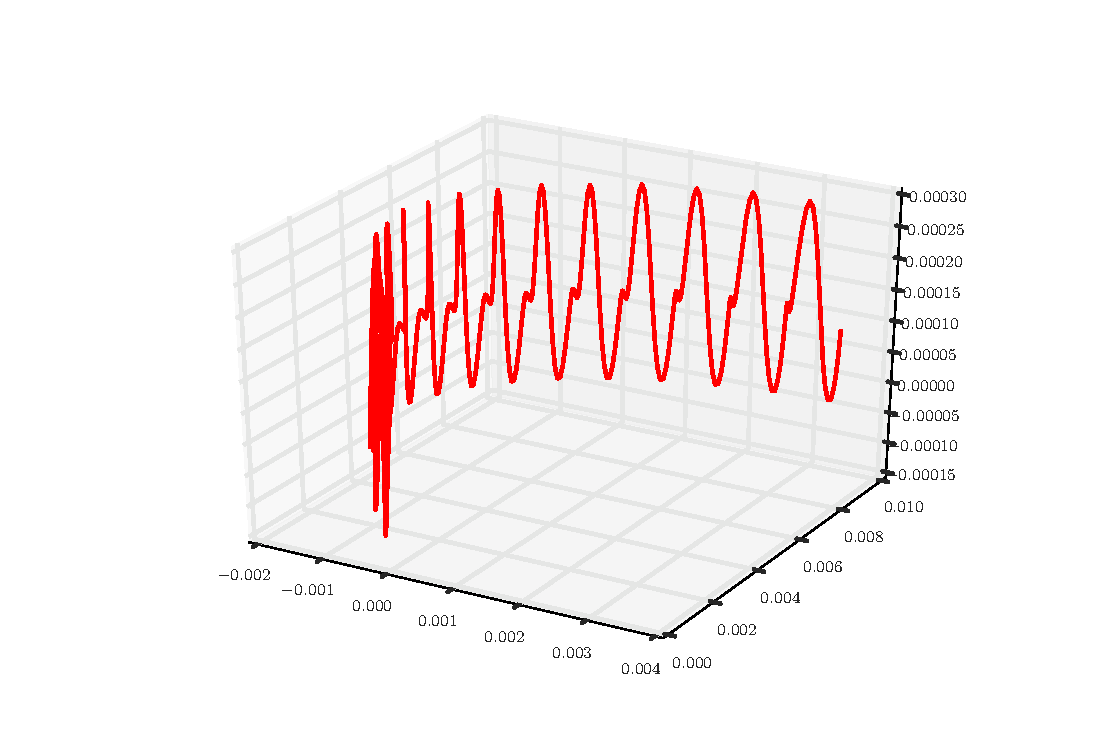
\includegraphics[width=0.49\textwidth]{../Figures/Behaviors/3d.pdf}
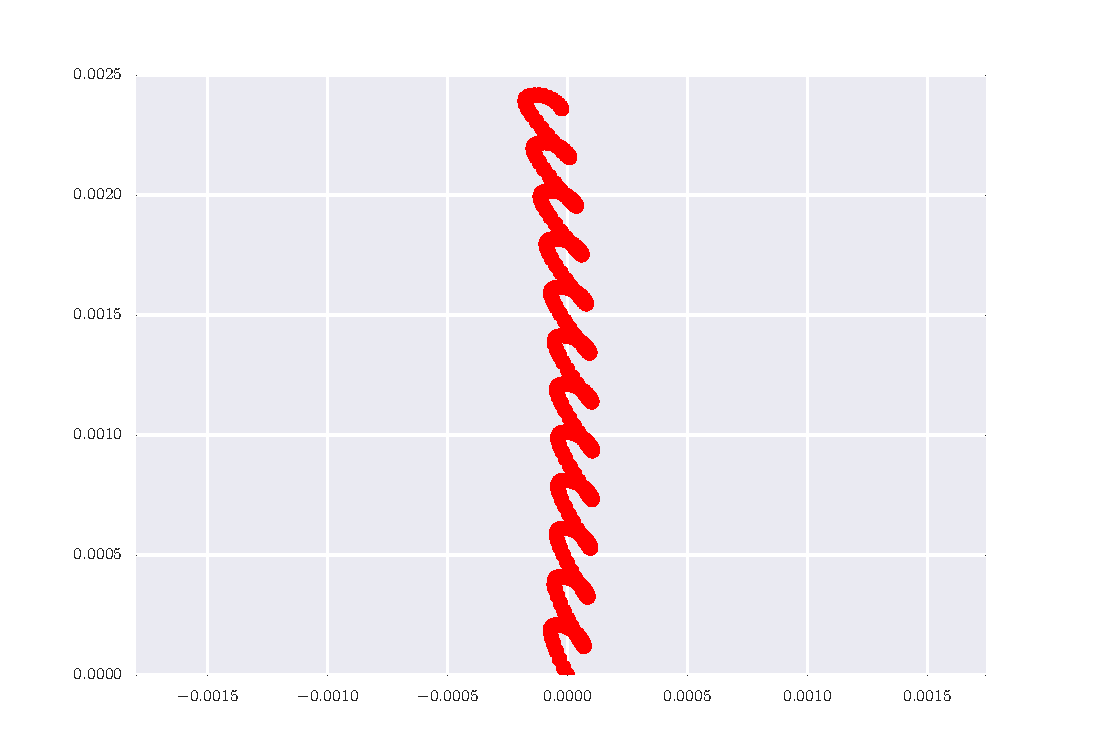
\includegraphics[width=0.49\textwidth]{../Figures/Behaviors/2d.pdf}
\caption{Three and two dimensional trajectories of the soft robots.}
\end{subfigure}
\vspace{-0.13cm}
\begin{subfigure}[b]{0.24\textwidth}
\centering
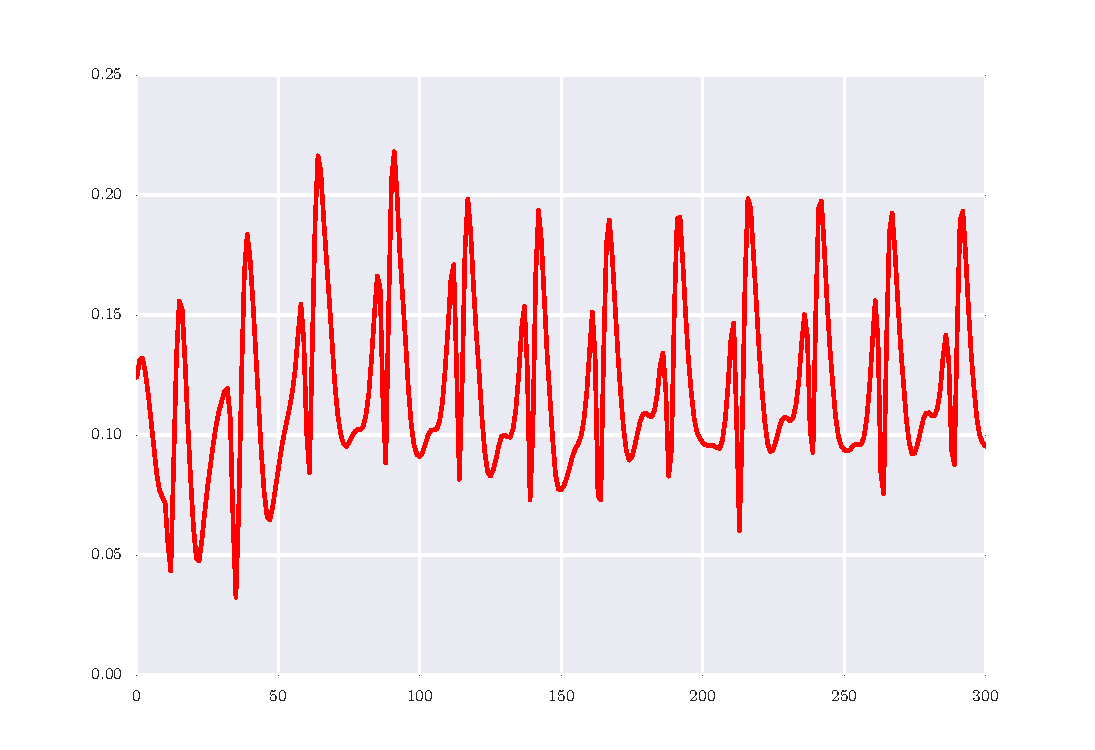
\includegraphics[width=0.49\textwidth]{../Figures/Behaviors/pace.pdf}~
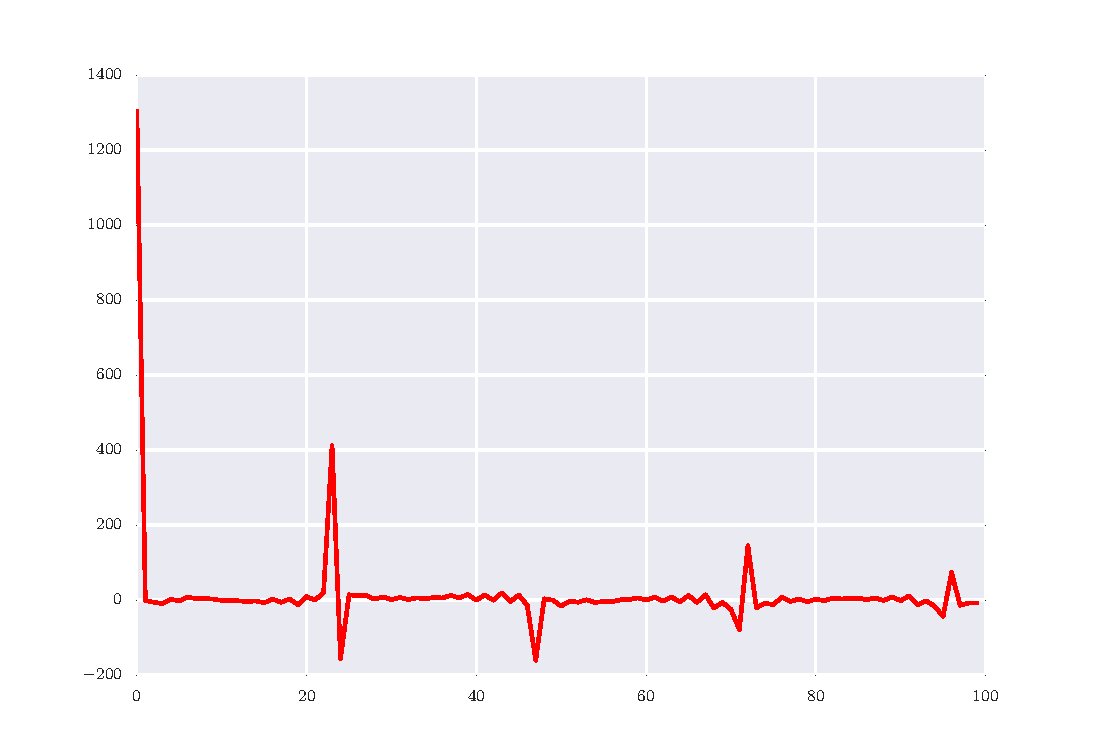
\includegraphics[width=0.49\textwidth]{../Figures/Behaviors/pacedft.pdf}
\caption{Pace and discrete Fourier transformation of the the same signal.}
\end{subfigure}~
\begin{subfigure}[b]{0.25\textwidth}
\centering
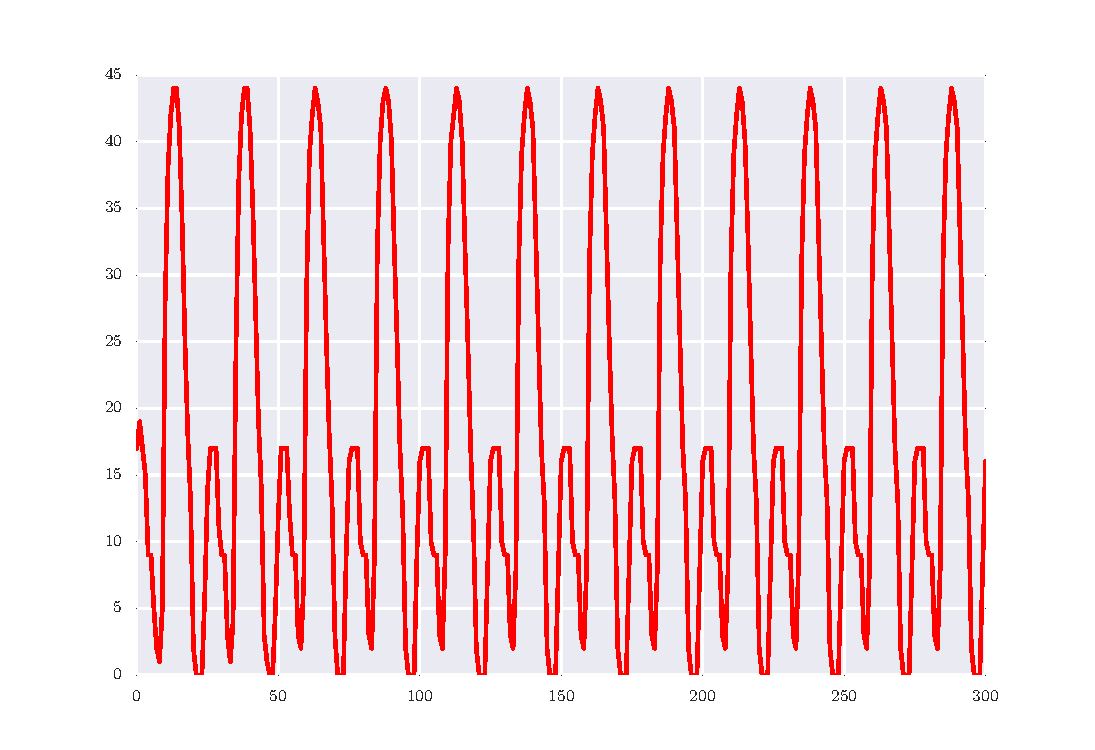
\includegraphics[width=0.49\textwidth]{../Figures/Behaviors/vtg.pdf}~
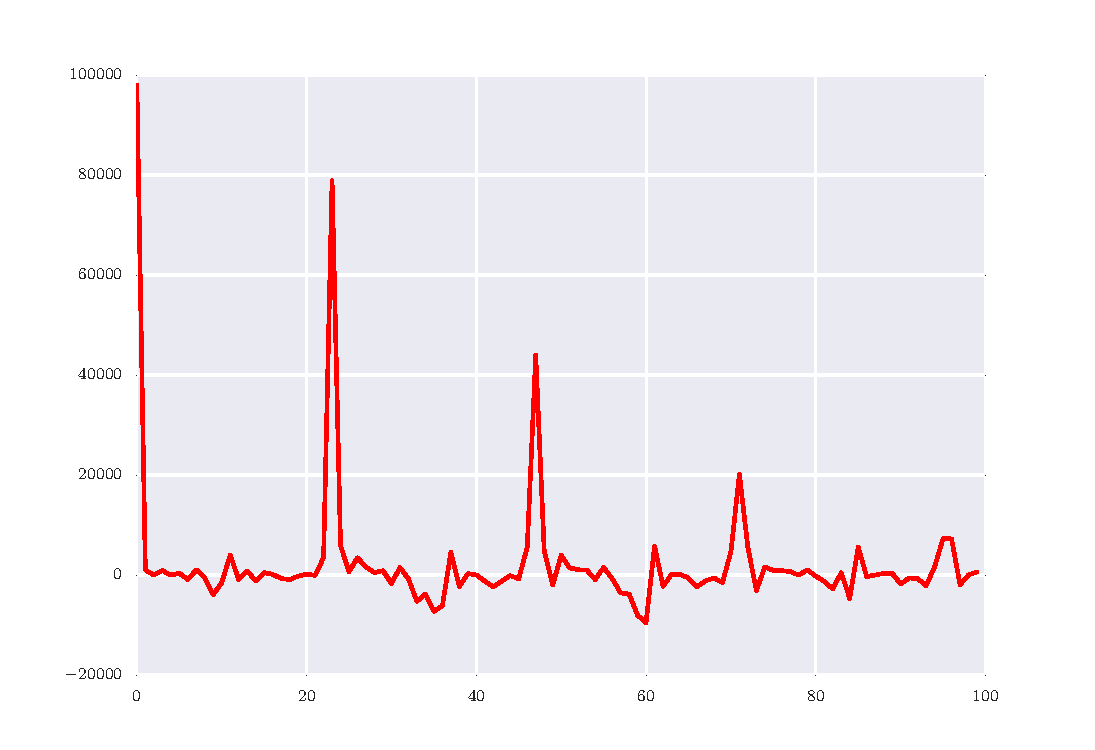
\includegraphics[width=0.49\textwidth]{../Figures/Behaviors/vtgdft.pdf}
\caption{Voxels touching the ground and discrete Fourier transformation of the the same signal.}
\end{subfigure}\\
\begin{subfigure}[b]{0.25\textwidth}
\centering
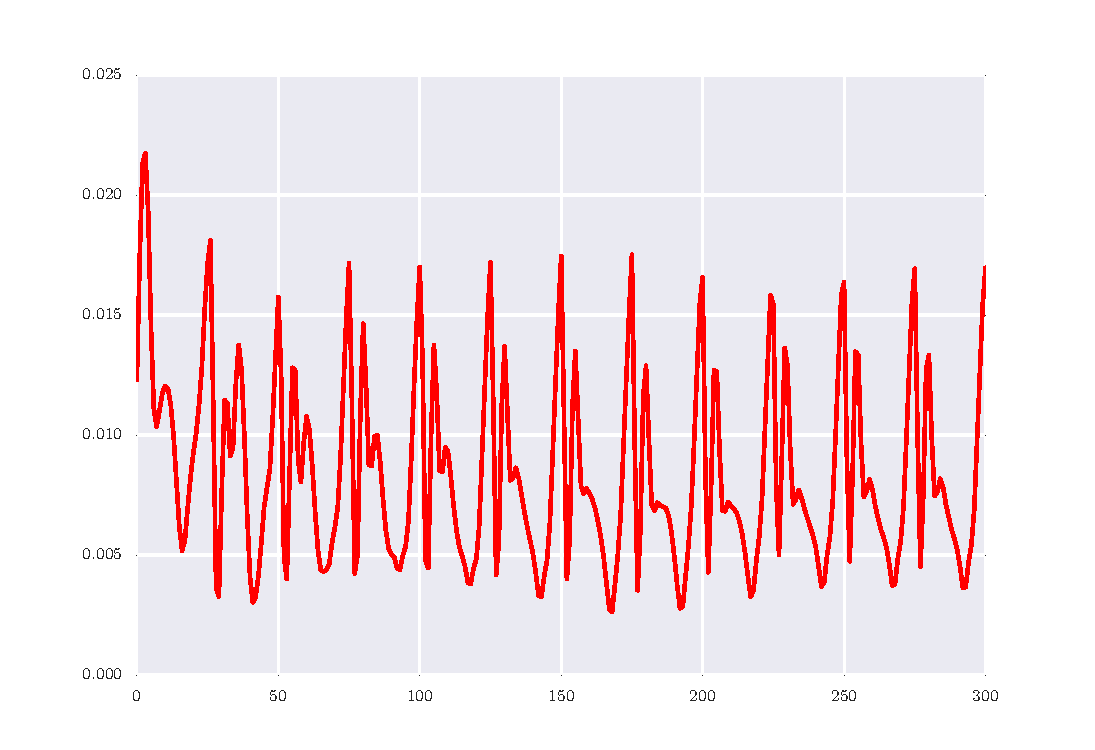
\includegraphics[width=0.49\textwidth]{../Figures/Behaviors/pr.pdf}~
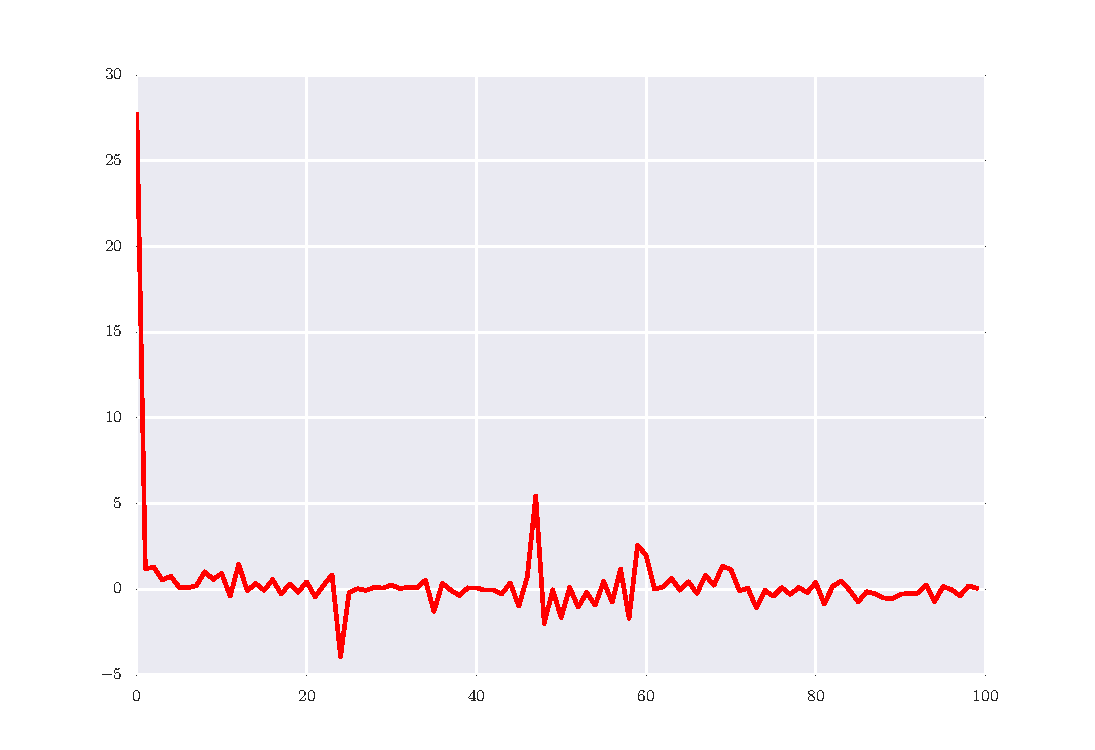
\includegraphics[width=0.49\textwidth]{../Figures/Behaviors/prdft.pdf}
\caption{Maximum pressure and discrete Fourier transformation of the the same signal.}
\end{subfigure}~
\begin{subfigure}[b]{0.25\textwidth}
\centering
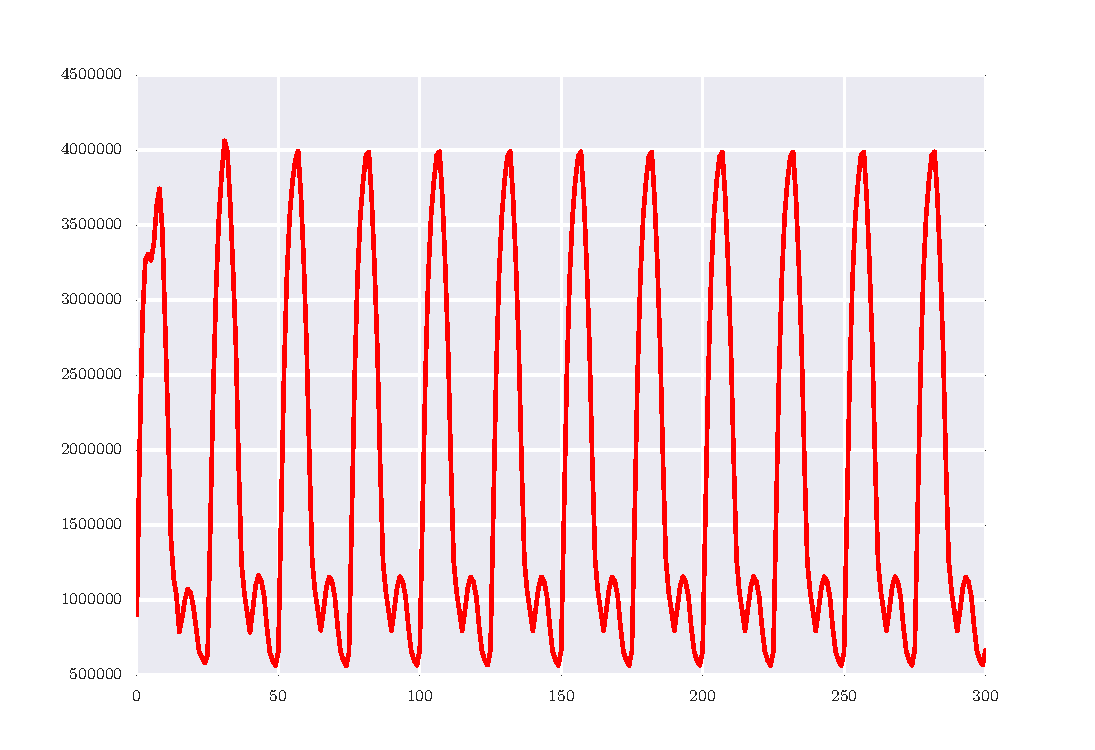
\includegraphics[width=0.49\textwidth]{../Figures/Behaviors/ke.pdf}~
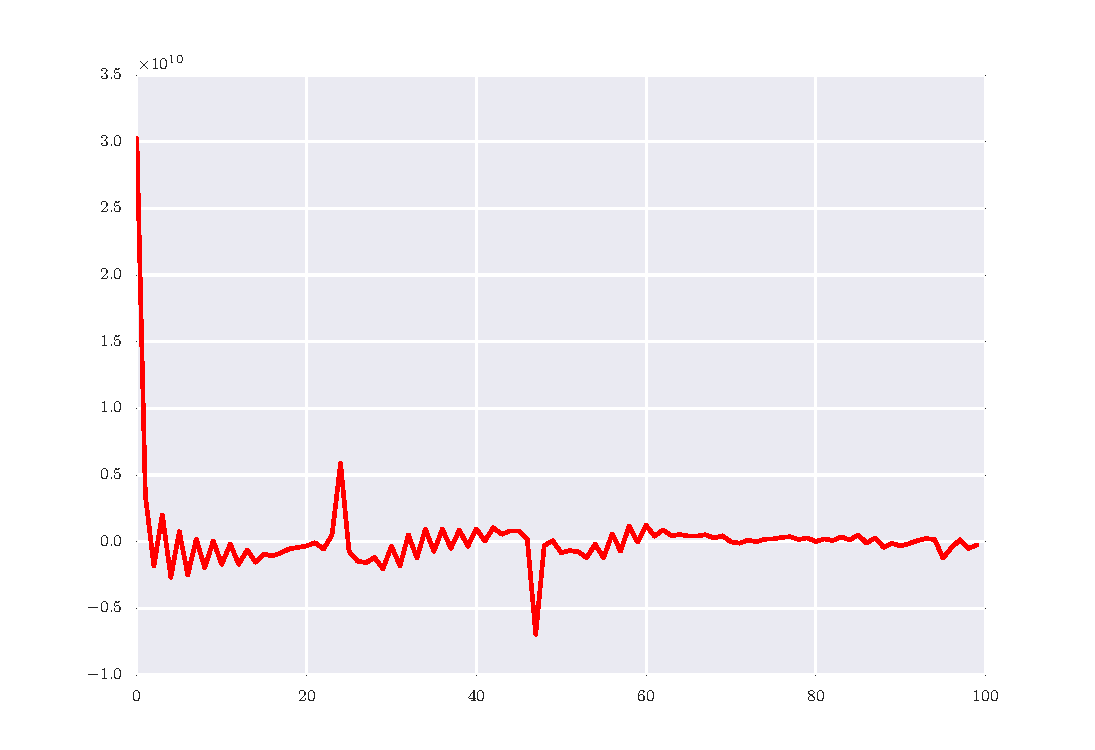
\includegraphics[width=0.49\textwidth]{../Figures/Behaviors/kedft.pdf}
\caption{Kinetic energy and discrete Fourier transformation of the the same signal.}
\end{subfigure}
\caption{Observed behaviors of the soft robots used for the sparsity computation in novelty search.}
\label{fig:Behaviors}
\vspace{-15pt}
\end{figure}

Regarding the evolution of soft robots in the specific simulated environment, a \emph{behavior} can be defined as the way soft robots interact towards the environment. Every aspect of the soft robots movement that can be observed can be used to describe their behavior. Previous work~\cite{lehman2011evolving} in a try to evolve walking three-dimensional virtual creatures used the evolved morphology of the creatures to describe their behavior. Although, comparing the morphology of the evolved soft robots is similar to comparing the chromosome (CPPN) of each individual. Behaviors that describe the morphology of the evolved robots have failed~\cite{lehman2011evolving}, since search is then forcing new types of morphologies without caring about the actual target of the evolution, which was the efficient locomotion. Therefore, only the comparison of the observed behavior in the phenotype level can lead the evolution towards more complex behaviors. 

It is expected that behaviors that contain information about the goodness (displacement) of individuals will be more successful than behaviors that include other aspects of the soft robots' behavior. Figure~\ref{fig:Behaviors} presents all the behavior types used for the novelty metric computation. For all recorder behavior metrics a constant sampling rate ensures that all signals have the same length. The behaviors designed to describe the strategy and the efficiency of the evolved locomotion strategies. They contain information that indirectly implies both the objectives of the evolution. \emph{Trajectories} (2D and 3D), incorporate all the needed information such as speed, displacement, and locomotion strategy. To avert from same trajectories in all possible directions trajectories are normalized, meaning that their starting coordinates are always the start of the axes ($<0,0,0>$) and the point coordinates of the trajectory are rotated so their center of mass is normalized to a specific angle ($\theta = 90^{o}$). To measure the difference of two trajectories the Euclidean distances between coordinates at the same sampling time are measured, so that:
\begin{align}
\text{i-trajectory: } &t_i = t_i^1, t_i^2, \ldots, t_i^N\\
\text{j-trajectory: } &t_j = t_j^1, t_j^2, \ldots, t_j^N\\
\text{Difference: } &t_i - t_j = \sum_{n=1}^{N} dist( t_i^n, t_j^n )
\end{align}
where $n$ is the number of sampled coordinate points and $dist$ is the Euclidean distance. Apart from trajectory type behaviors, pace, voxels touching the ground, kinetic energy, pressure, as well as, the discrete Fourier transformation of these signals were used to define other behavior types. The similarity or the difference of two of the same type behaviors can be determined by the equations provided while these measures of difference are used by the sparsity equation (see Eq.~\ref{sparsenessEquation}) to compute the sparseness of a given behavior in the behavior space. Individuals with novel observed behaviors (high sparseness value) are then stored in a list helping the evolution to avoid generating similar behaviors.


\subsection{Fitness Elitism in Novelty Search}

Elitism is the process of passing mutations or copies of the best individuals to the next generation. The best individuals of each species generation are protected so they can contribute with their beneficial genes later in the evolution. Novelty search can include elitism in its selection process, and it does that by copying the most novel organisms of the current population of each species to the next while the same function can also be used to copy fit individuals within novelty search method. The way these two elitism functions can be combined together depends on the population size and the problem, while probabilistic methods can also be applied. In the specific setting, both elitism function copy new individuals to the new generation with probability one. Moreover, evolution towards novelty does not get disturbed, at the same time fit individuals have the chance to be optimized further as long as they are the fittest within the species population. 

\subsection{Experimental setup}
Each experiment consists of $10$ runs under the same settings. As in~\cite{cheney2013unshackling} and for comparison purposes a population of $30$ on each generation is used, the maximum number of generations in the evolution is set to $1000$. Due to computationally expensive simulations, not all experiments are performed using a lattice resolution of $10^3$, resolutions lower than $10^3$ are used as well. More specifically, $5^3, 7^3, 10^3$ lattice resolutions are used. All settings regarding CPPN-NEAT algorithm are the same as in~\cite{cheney2013unshackling}.



\begin{figure}[b!]
\centering
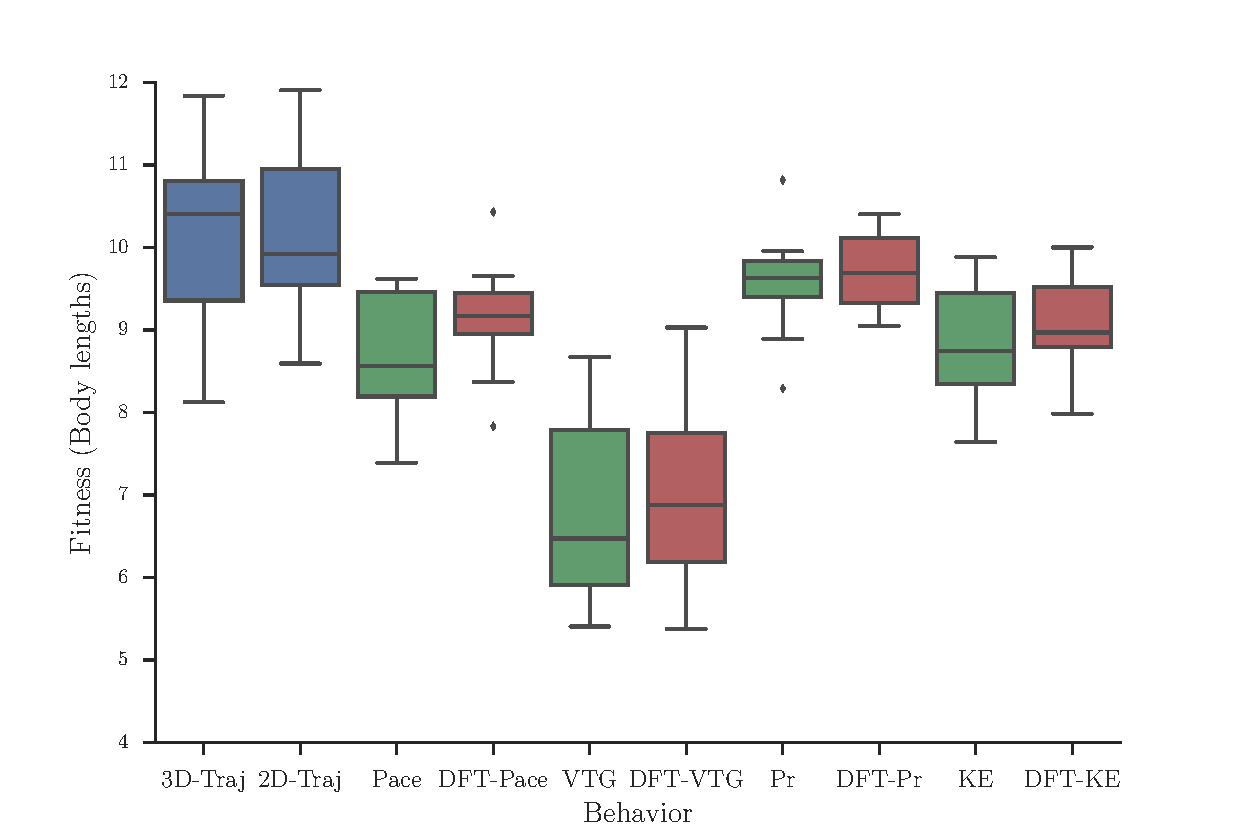
\includegraphics[width=0.5\textwidth]{../Figures/Results/BehaviorPerformanceNoveltyOnly.pdf}
\caption{Distributions of the champion fitness under $10$ variant defined behaviors for novelty search. \textcolor{RoyalBlue}{Blue} are trajectory type behaviors (3D and 2D), \textcolor{ForestGreen}{Green} are 1D signals (Pace, Voxels touvhing the ground (VTG), Pressure (Pr), and Kinetic energy (KE)). \textcolor{BrickRed}{Red} is the discrete Fourier transformation of these 1D signals.}
\label{fig:BehaviorsPerformance}
\vspace{-15pt}
\end{figure}

\section{Results}
Pure novelty search is compared in respect to the goodness measure used in the simulations (displacement of soft robots in body-lengths) to fitness based search. Different behavior types are used to investigate the effects on performance of novelty search method. Elitism is used in a proposed methodology to incorporate fitness information in novelty search. Last, the performance of both methods are investigated for several levels of gravity. Furthermore, evolved locomotion strategies under different gravity conditions show how environmental conditions can affect the evolved morphologies and the locomotion strategies of soft robots.

\begin{comment}
\subsection{Evolved Morphologies} 

Apart from the performance that the two methods achieved, both of them were successful in evolving effective strategies for the locomotion of the evolved morphologies. Figure~\ref{fig:evolvedMorphologiesFitness} shows three different gait types evolved by fitness based search. All of these morphologies are considered ``good'' in respect to their fitness value, meaning that they achieve to travel up to $\sim 10$ body lengths during the simulation time ($0.4$ sec.). Considering that the lattice resolution used for this experiment was of size $10^3$. The produced low-resolution soft robots cannot be compared with real-life organisms. However, the results are shown that even in such low dimensions life-like locomotion can be evolved. For the fitness based search, soft body morphologies can use their front leg(s) to pull themselves forward, evolve a four-leg locomotion where a nose and a tail are mostly used for stability, push and pull themselves forward, and gallop using both of their legs. Moving from fitness based search to novelty search locomotion strategies do not differ too much since the resolution does not allow the virtual soft robots to explore more locomotion techniques. However, novelty search proves its merits with regards to the morphologies evolved. More complicated structures are now evolved, this can be explained by the fact that novelty search pushes the evolution to investigate new kinds of behaviors resulting to more complex topologies for the networks (CPPNs) that represent the soft robot morphologies. Figure~\ref{fig:evolvedMorphologiesNovelty} presents four champion morphologies and their locomotion strategies. Two-legged galloping soft robots, animal-like locomotion based on four legs, and hopper soft robots are evolved.
\end{comment}


\subsection{Behavior selection} 

Figure~\ref{fig:BehaviorsPerformance} illustrates the performance achieved by novelty search for $10$ behavior types. What is shown is the fitness in body lengths of the champion soft robot of the whole evolution from $10$-independent runs. Both trajectory-type behaviors achieve the best performance in regards to the fitness measure, with a small difference in favor of two-dimensional over three-dimensional trajectories. The rest of the behavior metrics apart from VTG and DFT-VTG are close as far as the final performance of the evolution is concerned. One reason they fail to meet the trajectories' performance is the fact that although they keep track of cues that can describe the performance of the robot (speed/displacement), they cannot encode the direction of them. Soft robots having a circle trajectory can produce fast locomotion, in this case though, the measured displacement from their initial position remains low. Counting the number of voxels of a soft robot that touched the ground in every sampling timestep of the simulation, does not imply how fast the robot is moving. A fast moving robot that is hopping can have a similar behavior with a hopping robot that stays in the same position. On the contrary, using the trajectories of these two soft robots, the behaviors observed would have been highly variant.


\begin{figure}[b!]
\centering
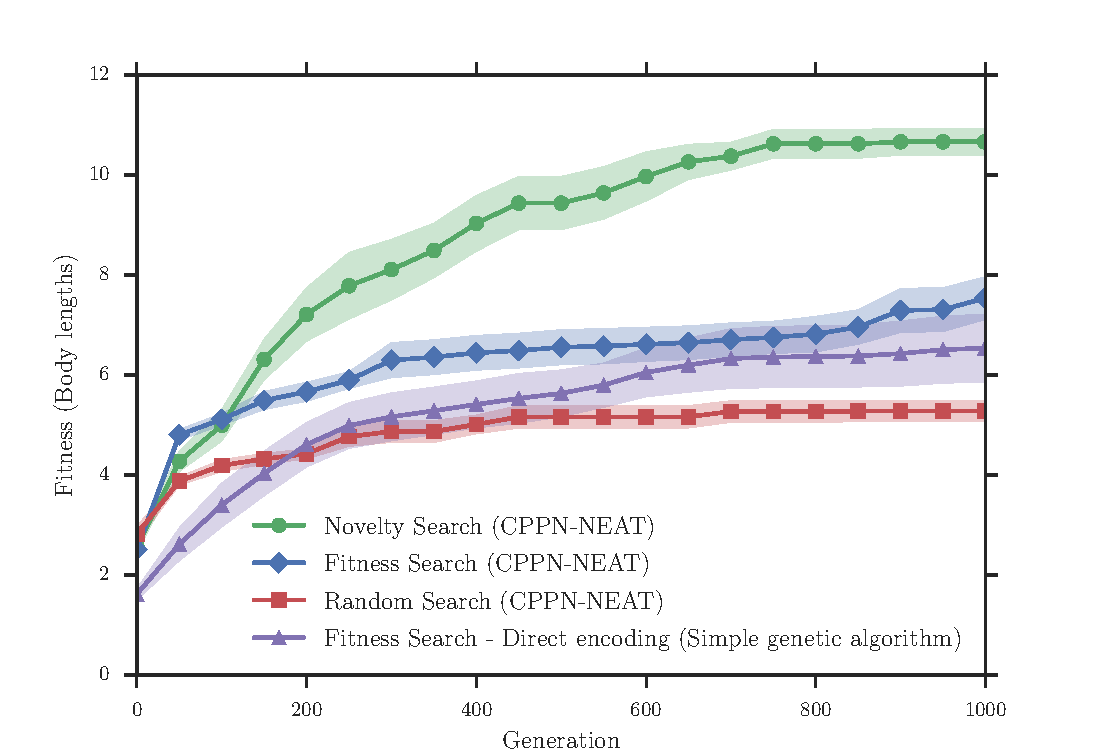
\includegraphics[width=0.5\textwidth]{../Figures/Results/FitNovRandomDirectSize5.pdf}
\caption{Comparison of simple genetic algorithm (direct encoding) against novelty-fitness-random search with generative encoding. Best fitness so far averaged over $10$ runs.}
\label{fig:FitNovRandomDirectSize5}
\vspace{-15pt}
\end{figure}

\subsection{Performance Comparison}

To compare the performance achieved by novelty search method, its performance is set side by side with fitness based search (normalized body-length displacement of the soft robot's center of mass from its initial position), random search, and finally a simple genetic algorithm\footnote{The GAlib C++ library \cite{wall1996galib} used for the implementation of this method. Source code used from~\cite{cheney2013unshackling}.} with direct encoded genomes. The same experiment held under two different simulation settings (for resolutions $5^3$ and $10^3$). Notice, that the first three methods are referring to a generative encoding (CPPNs) evolved by CPPN-NEAT evolutionary algorithm and using selection in respect to novelty, fitness, and random selection. The last method uses a direct encoded genome driven by fitness within a simple genetic algorithm. Two dimensional trajectories are used by novelty search in order to describe the novelty in the behavior space through sparsity equation.

\begin{figure}[t!]
\centering
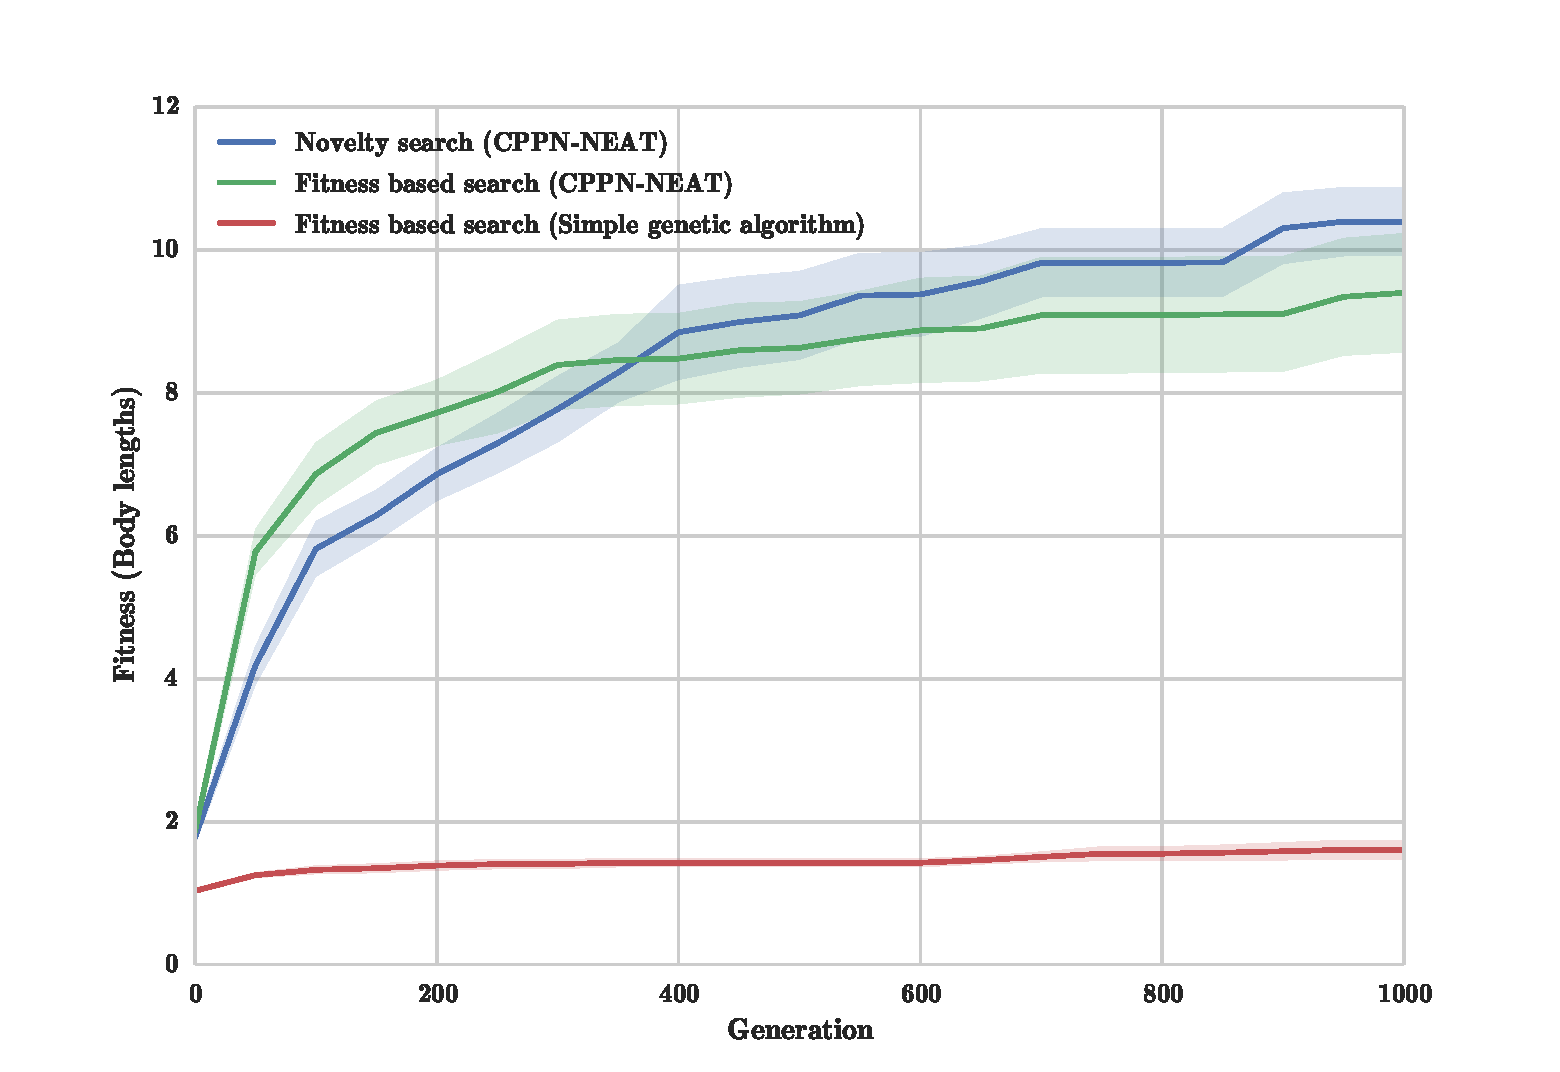
\includegraphics[width=0.5\textwidth]{../Figures/Results/FitvsNovVsDirSize10.pdf}
\caption{Comparison of simple genetic algorithm (direct encoding) against novelty-fitness-random search with generative encoding. Best fitness so far averaged over $10$ runs.}
\label{fig:FitvsNovVsDirSize10}
\vspace{-15pt}
\end{figure} 

Figure~\ref{fig:FitNovRandomDirectSize5} presents the results for the low resolution soft robots ($5^3$). The average best displacement so far is presented alongside the deviation error. Notice, the difference between novelty search and the other methods. Using the two-dimensional trajectories of the soft robots, novelty search visits optimal solutions that none of the other methods does. Local optima can prevent fitness based search to achieve the performance of novelty search. Encoding limitations in direct encoding cannot lead to optimal solutions for this settings. In the case of random search, having neither the information about their fitness, nor the driving force of novelty search that seeks for novel behaviors, it fails to evolve any decent locomotion. The only reason random search in CPPN-NEAT achieves to evolve displacement of $\sim 5$ body-lengths, is the powerful encoding used (CPPNs). The simple genetic algorithm approach performs better than using random selection with an indirect encoding. Structural regularity do not show all of their advantages in such low resolution settings.

In higher resolution lattices, it is expected that generative encoding will prove its merits over the direct encoding scheme~\cite{cheney2013unshackling,stanley2007compositional}. More complicated morphologies can be produced (morphology space for $10^3$ lattice resolution: $9.3 \times 10^{698}$). Furthermore, the space of behaviors, for instance two-dimensional trajectories, becomes larger since more complex soft robots can achieve higher displacement and more advanced strategies for locomotion. As it has been shown before, these higher resolution morphologies can achieve life-like locomotion. Figure~\ref{fig:FitvsNovVsDirSize10} illustrates the performance (i.e best displacement so far) of the four different methods in these higher resolution settings. Results reassure that novelty search achieves higher fitness ($> 1$-bodylength) on average against fitness based search. Nevertheless, there is no tremendous difference as in the previous experiment. Both methods achieve to evolve the soft robot structure with the highest fitness found in all experiments ($\sim 14$ Body lengths). Novelty search behaves more constant in evolving individuals with high fitness in all runs, on the other hand most of individual runs of fitness search are being trapped in low fitness local optima, trying to optimize specific individuals without trying to explore deeply the fitness landscape like novelty search successfully does. The high difference between random evolution and novelty search proves that seeking novel behaviors in novelty search cannot be considered as a random search. The superiority of generative encoding (CPPN) over direct encoding can be evidently observed. Regular in shape morphologies can take advantage of their geometrical properties to move efficiently.

\begin{figure}[t!]
\centering
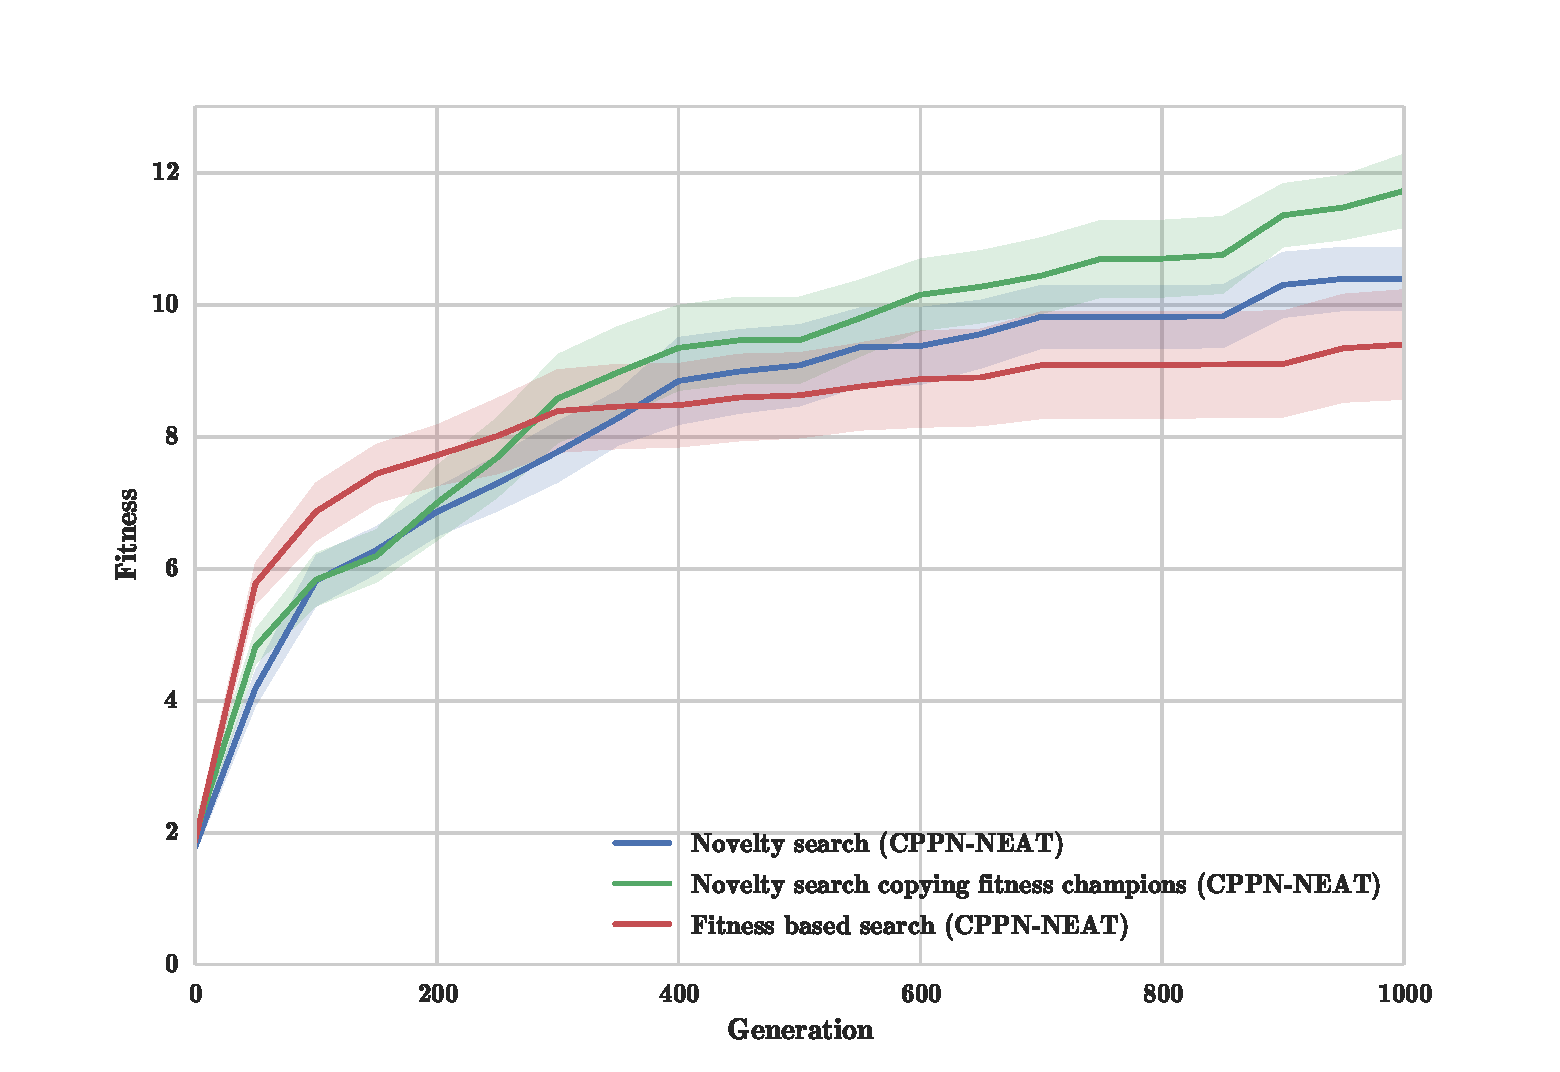
\includegraphics[width=0.5\textwidth]{../Figures/Results/CopyFitChampions10.pdf}
\caption{Best fitness so far, novelty search with and without copying \emph{fit} champions (Fitness Elitism), and fitness search, averaged over $10$ runs.}
\label{fig:CopyFitChampions10}
\vspace{-15pt}
\end{figure}


\subsection{Fitness Elitism in Novelty Search}

The reason that novelty search is considered such a revolutionary search method is because it finds solutions for deceptive problems, where the fitness landscape is not a straightforward function. On each generation of novelty search novel behaviors that are also fit in regards to the objective of the problem are discovered. Mutations of these solutions will yield in behaving similarly to their ancestors, resulting in similar behaviors. Thus, the novelty value of these individuals will be declined as similar behaviors will contribute in a denser area in the behavior space. Eventually, these solutions will stop being selected, and evolution will not have the chance of carrying their genes along. Mutations and other genetic operations can optimize these fit individuals more. These individuals (with high fitness value) can be seen as \emph{stepping~stones}~\cite{lehman2011abandoning} towards more optimized versions of themselves. Being blind to the objective function, novelty search will eventually stop producing new individuals out of them, which will lead to promising individuals being unable to survive through the evolution process. Figure~\ref{fig:CopyFitChampions10} illustrates the gain in performance when fitness elitism is used in novelty search method compared with the pure novelty and fitness based search methods.


\section{Evolving Soft Robots for Outer Space} 

\begin{figure}[b!]
\centering
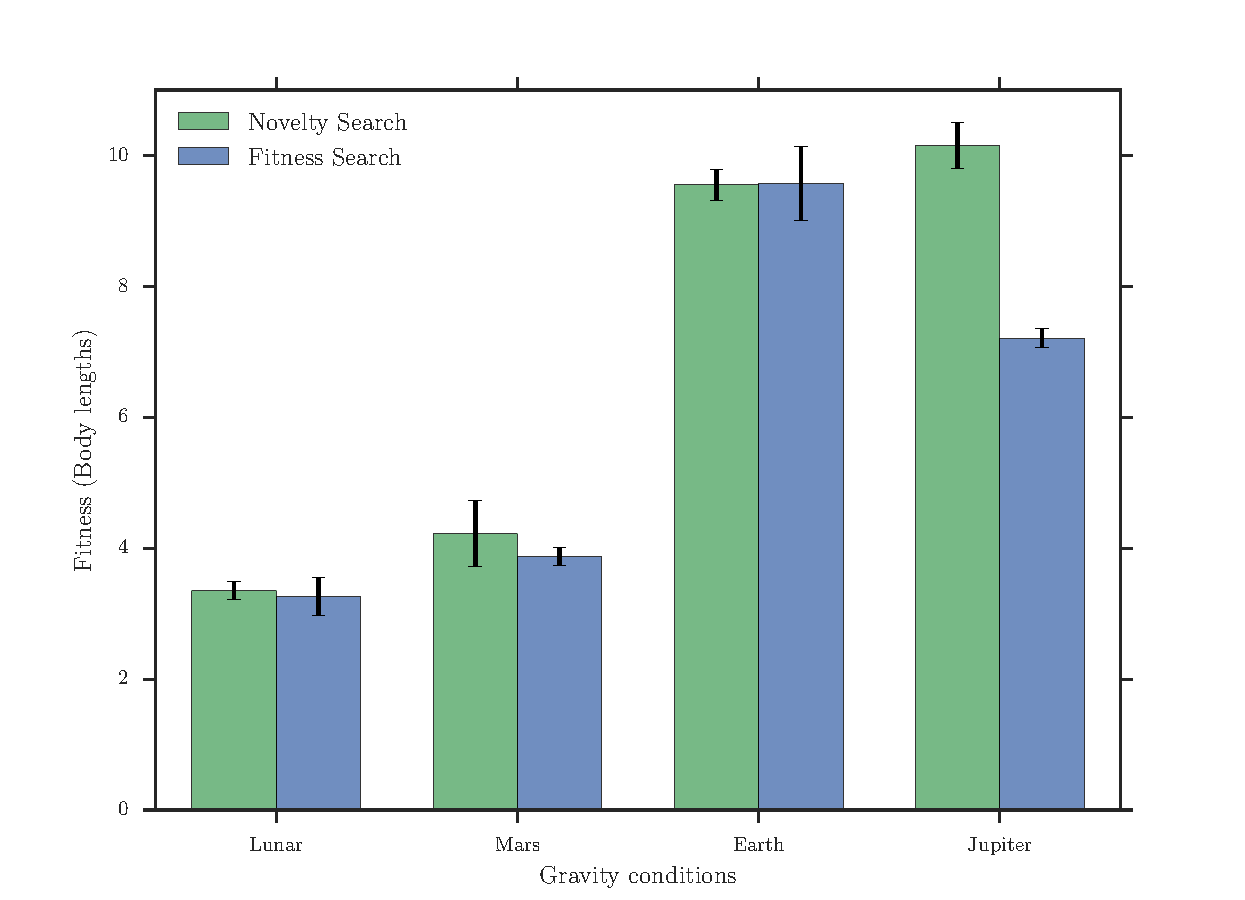
\includegraphics[width=0.5\textwidth]{../Figures/Results/GravityExperiment.pdf}
\caption{Novelty search performs better or equally good than fitness based search in all gravity conditions tested.}
\label{fig:gravityConditions}
\vspace{-15pt}
\end{figure}


Gravity conditions can affect the evolution of soft robots. Both methods discussed, novelty and fitness based search, are used for the co-evolution of the morphology and the locomotion strategy of soft robots under variant gravity levels. For the novelty search method two-dimensional trajectories of the soft bodies are chosen as the behavior metric to evaluate the novelty of each individual. Figure~\ref{fig:gravityConditions} presents the performance of novelty and fitness based search for four different gravity levels under a lower resolution setting of $7^3$.

\begin{figure*}[t!]
\centering
\begin{subfigure}[b]{1.0\textwidth}
\centering
\foreach \i in {2,3,4,5,6,8,9}{ 
\includegraphics[width=0.14\textwidth]{../Figures/Robots/moon-nov-g1-2-\i.jpg}\hspace{-0.16cm}
}
\caption{\textbf{Lunar }C-shaped hopper (Novelty-Search)}
\label{fig:gravityRobots1.6-4}
\end{subfigure}
\begin{subfigure}[b]{1.0\textwidth}
\centering
\foreach \i in {1,2,3,4,5,7,8}{ 
\includegraphics[width=0.14\textwidth]{../Figures/Robots/mars-nov-g3-1-\i.jpg}\hspace{-0.16cm}
}
\caption{\textbf{Mars }2-legged C-shaped hopper (Novelty-Search)}
\label{fig:gravityRobots3.7-2}
\end{subfigure}
\begin{subfigure}[b]{1.0\textwidth}
\centering
\foreach \i in {1,2,3,4,5,6,7,8,9,10}{ 
\includegraphics[width=0.097\textwidth]{../Figures/Robots/grass-fit-g9-2-\i.jpg}\hspace{-0.16cm}
}
\caption{\textbf{Earth }\emph{Top view}, 4-legged animal like locomotion (Fitness-Search)}
\label{fig:gravityRobots9.8-2}
\end{subfigure}
\begin{subfigure}[b]{1.0\textwidth}
\centering
\foreach \i in {1,2,3,4,5,7,8}{ 
\includegraphics[width=0.14\textwidth]{../Figures/Robots/grass-nov-g9-1-\i.jpg}\hspace{-0.16cm}
}
\caption{\textbf{Earth }Tumbleweed-like locomotion (Novelty-Search)}
\label{fig:gravityRobots9.8-3}
\end{subfigure}
\begin{subfigure}[b]{1.0\textwidth}
\centering
\foreach \i in {1,2,3,7,8,9,10}{ 
\includegraphics[width=0.14\textwidth]{../Figures/Robots/gas-nov-g2-1-\i.jpg}\hspace{-0.16cm}
}
\caption{\textbf{Jupiter }(Assuming a stable surface) C-shaped hopper (Novelty-Search)}
\label{fig:gravityRobots27.6-3}
\end{subfigure}
\caption{Locomotion strategies evolved in variant gravity conditions.}
\label{fig:gravityRobots1.6}
\vspace{-15pt}
\end{figure*}

\subsubsection*{Robots on Lunar}

Locomotion strategies evolved under low gravity conditions for the gravity of the Lunar more specifically, showed that only hopping gaits can produce effective locomotion. Low gravity makes it difficult for the soft body structures to grip on the ground surface and evolve different strategies than hopping. The morphology of each hopper differs. A C-shaped hopper soft robot (see Fig.~\ref{fig:gravityRobots1.6-4}) evolved in these settings.

\subsubsection*{Soft Robots on Mars}

The locomotion effectiveness on Mars is higher when is compared to this on Lunar's gravity acceleration making it possible for the virtual soft robots to evolve other kind of gaits using legged bodies (see Fig.~\ref{fig:gravityRobots3.7-2}). Note that the C-shaped hopper soft robot mostly uses passive materials apart from its upper body where all the active material are located. With using its upper part generates enough motion able to move itself. What is observed in the morphologies of soft robots evolved in lower gravity levels was that the use of less number of active voxels can produce decent locomotion.

\subsubsection*{Soft Robots on Earth}

On higher gravity levels life-like locomotion emerges. Interesting animal-like gait has been evolved (see Fig.~\ref{fig:gravityRobots9.8-2}) verifying the connection there is between gravity and the locomotion strategies of living organisms evolving on Earth for thousands of years. Tumbleweed-like locomotion (see Fig.~\ref{fig:gravityRobots9.8-3}) has been emerged under novelty search method producing rolling soft robots that can locomote efficiently. Fact that adds significance to the novelty search method since fitness based search did not produce this kind of locomotion strategy. Tumbleweed is a concept of low-cost exploration that has inspired robot designers for Mars' missions in the past~\cite{antol2003low} and has been already deployed in Antarctica for testing purposes by NASA.

\subsubsection*{Soft Robots on Jupiter}

Moving on to higher gravity levels, Jupiter, heavier structures can use galloping as a strategy for their locomotion. Galloping is again considered to be an effective way of moving in such a high gravity, whereas thicker legs are evolved to withstand the high gravitational force. Push-pull worm-like locomotion can also produce decent velocities for soft robots. Finally, hoppers have also been evolved to this setting, while they are using more actuated materials (see Fig.~\ref{fig:gravityRobots27.6-3}).


Different locomotion strategies can be evolved on different gravity levels producing effective locomotion. Low gravity does not allow other kinds of locomotion apart from hoppers to be evolved, while higher gravity acceleration allows more complicated behaviors to be evolved. In all settings, both search methods produced effective locomotion for the soft body structures, however, the performance in regard to the objective measure defined, displacement of the body in body lengths, was equal or higher for novelty search in all gravity settings.

\begin{figure}[t!]
\centering
\vspace{-0.13cm}
\begin{subfigure}[b]{0.5\textwidth}
\centering
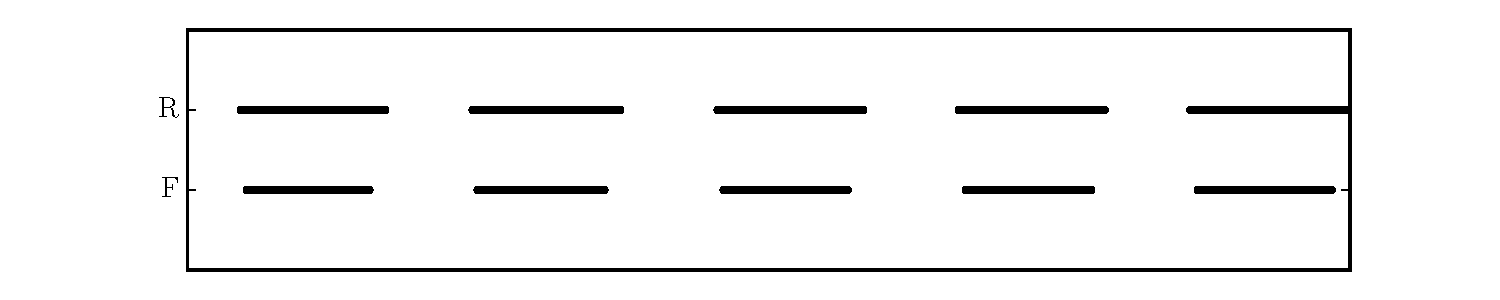
\includegraphics[width=1.0\textwidth]{../Figures/Results/hildebrand1.pdf}
\caption{Two legged soft robot. Timing of impacts between its legs and the ground.}
\end{subfigure}
\vspace{-0.13cm}
\begin{subfigure}[b]{0.5\textwidth}
\centering
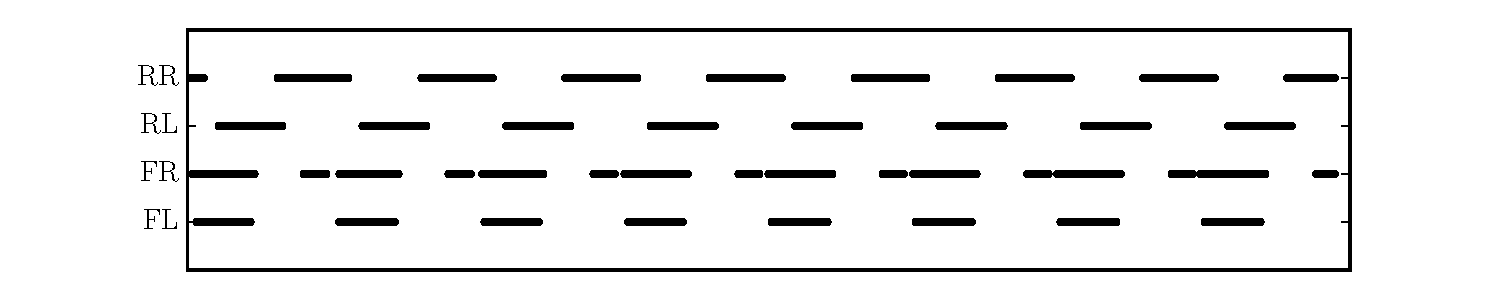
\includegraphics[width=1.0\textwidth]{../Figures/Results/hildebrand2.pdf}
\caption{Four legged soft robot. Timing of impacts between its legs and the ground.}
\end{subfigure}
\vspace{-0.13cm}
\caption{Hildebrand diagrams of two evolved soft robots for Earth's gravity acceleration.}
\label{fig:hildebrand}
\vspace{-15pt}
\end{figure}

\section{Discussion}
what's the use of this?
getting inspiration for soft robotic probe / landers (tumbleweed)
come back to asteroid scenario (passime motion), would it have saved Philae?
\begin{comment}
Experiments under these gravity levels verified that novelty search is indeed performing better than fitness based search in the evolution towards high-velocity soft robots in this setting. In addition, some interesting characteristics of evolved locomotion strategies under variant gravity condition were also observed, adding knowledge and more possibilities when the gait of a soft robot under low or high gravity is considered. With the progress three-dimensional printing is showing, future space missions can benefit from low cost soft robot explorers evolved to produce efficient locomotion. Passive locomotion can add more value to these soft body structures, where environmental variable conditions can actuate certain material types to produce locomotion.
\end{comment}


\section{Conclusions}
For the first time in evolutionary soft robotics a diversity based method such as novelty search was used. Novelty search method outperformed traditional fitness based search in evolving soft robots morphologies under the same objective which was the normalized by body-length displacement of soft robots. Previous work in evolving virtual creatures by novelty search~\cite{lehman2011evolving} used the resulted morphology of the robots created to determine the novelty of an individual. The resulted performance for pure novelty search method was worse than the fitness based. On the contrary, well defined behavior metrics can lead novelty search to outperform traditional fitness based search used in~\cite{cheney2013unshackling}. Novelty search not only improved the performance and the diversity in the behavior space, but also contributed to a larger variety of virtual creatures evolved. Incorporating fitness information in novelty search resulted in a significant performance gain over pure novelty search method. Finally, both techniques were used to evolve soft robots in four variant gravity levels, showing interesting results and the possibility of influencing future robotic designs for planetary exploration.

\subsection{Future Work}
ensamble of behaviors, very low gravity environments and rotational parameters of small body linked to actuation frequency


\begingroup
\setstretch{0.8}
\bibliographystyle{abbrv}
\bibliography{bibliography}
\endgroup
\end{document}
